\section{Submissions}

The competition was announced on 2013-01-15 at the Early Symmetric Crypto workshop in Mondorf-les-Bains, also announced online\footnote{\url{https://groups.google.com/d/forum/crypto-competitions}}. First-round submission papers must have been received till 2014-03-15, reference software implementations must have been received till 2014-04-15.

After passing the first-round deadline, all submissions were published. All submission papers can be downloaded on CAESAR homepage\footnote{\url{http://competitions.cr.yp.to/caesar-submissions.html}}. Submission source codes are bundled together with SUPERCOP benchmark application\footnote{\url{http://bench.cr.yp.to/supercop.html}}. There is a website with SUPERCOP speed benchmark results\footnote{\url{http://www1.spms.ntu.edu.sg/~syllab/speed/}}.

Also there was Directions in Authenticated Ciphers (DIAC) 2014 conference, where a lot of sumbission authors presented their candidates. Talk slides are available for download on the DIAC website\footnote{\url{http://2014.diac.cr.yp.to/index.html}}.

There were submitted 57 candidates for the CAESAR competition. A good insight into their classification is provided by Authenticated Encryption Zoo\footnote{\url{https://aezoo.compute.dtu.dk/}}. At the time of writing this thesis, 9 candidates (AES-COBRA, Calico, CBEAM, FASER, HKC, Marble, McMambo, PAES and PANDA) are considered broken and were withdrawn from the competition, because a cryptanalysis was published that broke the security claim made by the designers. \cite{cryptoeprint:2014:792} There are 48 candidates remaining. It is expected that the about a half of them will advance to the second round.

Announcement of second-round candidates was initially scheduled for 2015-01-15. However it is a hard task to do a proper security review, analysis and comparison of all submissions. Currently in the time of writing this thesis, the second-round candidates announcement is being postponed every month.


\subsection{Overall construction}

\begin{figure}
  \centering
  \begin{minipage}{0.8\textwidth}
    \raggedleft
    \begin{tikzpicture}
      \node (table) [matrix,row sep=1.5*\nodeheight,column sep=\nodeheight] {
        \node (plaintext1) [smallrect] {$m_1$}; & \node (plaintext2) [smallrect] {$m_2$}; & \node (plaintext3) [smallrect] {$m_3$}; \\
        \node (encryption1) [circle] {$E_K$}; & \node (encryption2) [circle] {$E_K$}; & \node (encryption3) [circle] {$E_K$}; \\
        \node (ciphertext1) [smallrect] {$c_1$}; & \node (ciphertext2) [smallrect] {$c_2$}; & \node (ciphertext3) [smallrect] {$c_3$}; \\
      };
      \path [line] (plaintext1) -- (encryption1);
      \path [line] (plaintext2) -- (encryption2);
      \path [line] (plaintext3) -- (encryption3);
      \path [line] (encryption1) -- (ciphertext1);
      \path [line] (encryption2) -- (ciphertext2);
      \path [line] (encryption3) -- (ciphertext3);

      \node (table2) [matrix,right=1 of table,row sep=\nodeheight,column sep=\nodeheight] {
        \node (plaintext) {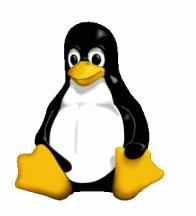
\includegraphics[scale=0.25]{images/tux.jpg}}; \\
        \node (ciphertext) {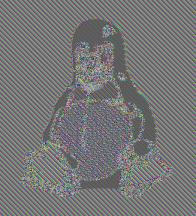
\includegraphics[scale=0.25]{images/tux-ecb.jpg}}; \\
      };
      \path [line] (plaintext) -- (ciphertext);
    \end{tikzpicture}
    \subcaption{ECB block mode}
  \end{minipage}
  \begin{minipage}{0.8\textwidth}
    \raggedleft
    \begin{tikzpicture}
      \node (table) [matrix,row sep=1.5*\nodeheight,column sep=\nodeheight] {
        \node (iv) [smallrect] {$IV$}; & \node (plaintext1) [smallrect] {$m_1$}; & \node (plaintext2) [smallrect] {$m_2$}; & \node (plaintext3) [smallrect] {$m_3$}; \\[-0.75*\nodeheight]
        & \node (plaintext1_after) [inner sep=0] {\Large $\oplus$}; & \node (plaintext2_after) [inner sep=0] {\Large $\oplus$}; & \node (plaintext3_after) [inner sep=0] {\Large $\oplus$}; \\[-0.75*\nodeheight]
        & \node (encryption1) [circle] {$E_K$}; & \node (encryption2) [circle] {$E_K$}; & \node (encryption3) [circle] {$E_K$}; \\[-0.75*\nodeheight]
        & \coordinate (ciphertext1_before) [inner sep=0]; & \coordinate (ciphertext2_before) [inner sep=0]; & \coordinate (ciphertext3_before) [inner sep=0]; \\[-0.75*\nodeheight]
        & \node (ciphertext1) [smallrect] {$c_1$}; & \node (ciphertext2) [smallrect] {$c_2$}; & \node (ciphertext3) [smallrect] {$c_3$}; \\
      };
      \path [line] (plaintext1) -- (plaintext1_after);
      \path [line] (plaintext2) -- (plaintext2_after);
      \path [line] (plaintext3) -- (plaintext3_after);
      \path [line] (plaintext1_after) -- (encryption1);
      \path [line] (plaintext2_after) -- (encryption2);
      \path [line] (plaintext3_after) -- (encryption3);
      \path [line] (encryption1) -- (ciphertext1);
      \path [line] (encryption2) -- (ciphertext2);
      \path [line] (encryption3) -- (ciphertext3);
      \path [line] (iv) |- (plaintext1_after);
      \path [line] (ciphertext1_before) -| ($(encryption1) !.5! (encryption2)$) |- (plaintext2_after);
      \path [line] (ciphertext2_before) -| ($(encryption2) !.5! (encryption3)$) |- (plaintext3_after);

      \node (table2) [matrix,right=1 of table,row sep=\nodeheight,column sep=\nodeheight] {
        \node (plaintext) {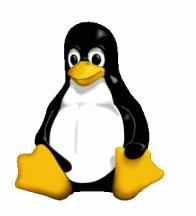
\includegraphics[scale=0.25]{images/tux.jpg}}; \\
        \node (ciphertext) {
\includegraphics[scale=0.25]{images/tux-cbc.jpg}}; \\
      };
      \path [line] (plaintext) -- (ciphertext);
    \end{tikzpicture}
    \subcaption{CBC block mode}
    \bigskip
  \end{minipage}

  \begin{footnotesize}
    The ECB mode is the most basic block mode, which does not perform any block feedback. Note that the plaintext structure is still observable in the ciphertext.
  \end{footnotesize}

  \caption{Basic block modes}
  \label{figure/block-modes}
\end{figure}

\begin{figure}
  \begin{minipage}{\textwidth}
    \centering
    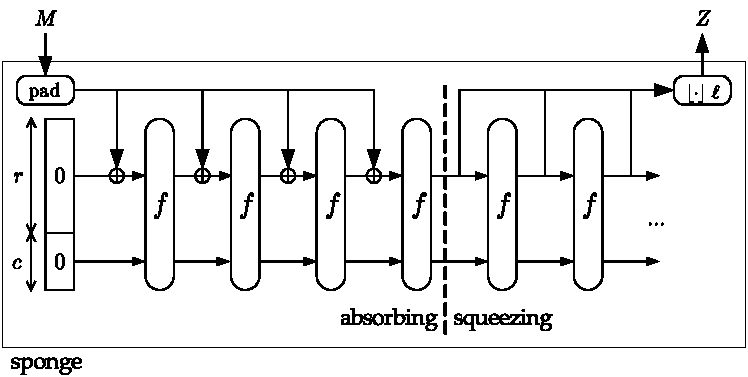
\includegraphics[scale=0.8]{images/sponge.pdf}
    \subcaption{The sponge construction}
  \end{minipage}
  \begin{minipage}{\textwidth}
    \centering
    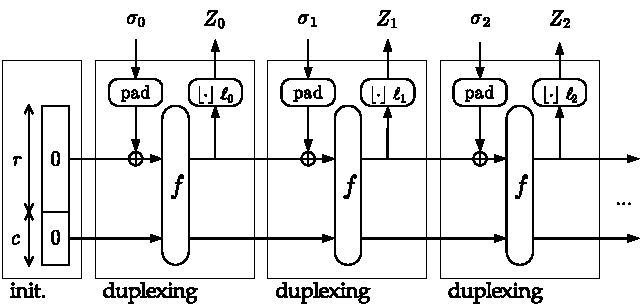
\includegraphics[scale=0.8]{images/duplex.pdf}
    \subcaption{The duplex construction}
  \end{minipage}

  \caption{Sponge functions}
  \label{figure/sponge-functions}
\end{figure}


Most of first-round candidates can be classified according to their construction design approaches. \cite{cryptoeprint:2014:792}

\begin{description}
  \item[Block Cipher] A block cipher is a bijective keyed permutation $E: \{0, 1\}^k \times \{0, 1\}^n \rightarrow \{0, 1\}^n, E(K, P) = C$, parametrized by a secret key $K$ of length $k$, and that takes as input a plaintext message $p$ of length $n$, and outputs a ciphertext message $c$ of length $n$. The permutation is used for encryption, an inverted permutation is used for decryption. A block mode is usually accompanied with a block mode.
  \begin{description}
    \item[Block Mode] A block mode (also called mode of operation) is used by block ciphers for secure transformation of data larger than a single block. See \autoref{figure/block-modes} for basic block modes. Some submissions defines only a new block mode and relies on existing block cipher (e.g. AES). \cite{cryptoeprint:2014:186} \\
    Example candidates: COBRA, JAMBU, POET
  \end{description}
  \item[Stream Cipher] A stream cipher is a pseudo-random generator, that takes a fixed-length secret key and generates a keystream of variable length. The keystream is combined with the plaintext message to produce ciphertext message and vice versa. The combining operation is usually XOR. \\
  Example candidates: ACORN, Morus
  \item[Key-Less Permutation] A key-less permutation is a bijective permutation on fixed-length strings. The key is sent to the permutation alongside the input, thus changing the internal state, effectivelly encrypting the output and producing the MAC tag.
  \begin{description}
    \item[Sponge Function] A sponge function is a generalization of both hash functions, which have a fixed output length, and stream ciphers, which have a fixed input length. It is a simple iterated construction for building a function with variable-length input and arbitrary-length output based on a fixed-length permutation. The inner permutation operates on a finite state of $b = r + c$ bits. The value $r$ is called the bitrate and the value $c$ the capacity. The sponge construction operates on the state by iteratively applying the inner permutation to it, interleaved with the entry of input or the retrieval of output, chunked by bitrate size. Literally, the sponge is said to \textit{absorb} its inputs block by block first before it processes and \textit{squeezes} it out afterwards. \cite{sponge-functions} \\
    A duplex sponge construction is closely related to the sponges. However unlike sponges, which are stateless between calls, the duplex construction allows alternation of input and output blocks at the same rate, like a full-duplex communication. Which means that it requires only one call of the inner permutation per input block. \cite{duplex-functions} See \autoref{figure/sponge-functions} for comparison. \\
    Example candidates: Ascon, ICEPOLE, Keyak, NORX, STRIBOB
  \end{description}
\end{description}


\subsection{Underlying primitive}

Under the overall construction usually hides a cryptographic primitive (e.g. inner permutation in sponge construction), which does the heavy lifting.

\begin{description}
  \item[AES] A lot of submissions use AES cipher or some of its parts (e.g. its round function), because during the years, AES have been enormously analysed in detail, and it is still believed to be secure. Moreover, starting with Intel's Westmere microarchitecture in 2011, current processors provide AES native instructions (AES-NI), that allow hardware-accelerated fast constant-time encryption and decryption.
  \item[Other named primitive] e.g. SHA2, Keccak, ChaCha, Streebog, etc.
  \item[Generic primitive type] e.g. Linear Feedback Shift Register (LSFR), Addition Rotation XOR (ARX), Logic Rotation XOR (LRX), Substition Permutation Network (SPN), etc.
\end{description}


\subsection{Functional characteristics, selection criteria}

The selection of second-round candidates will focus not only on general security of the scheme, but no less on important functional characteristics, which are good to have.

\begin{description}
  \item[High Security] The schema should be secure against all known kinds of cryptanalysis.
  \item[High Speed] The schema should be fast enough to compete with existing ciphers. However it is arguable whether the speed can be achieved by hardware acceleration such as by AES-NI or SIMD (SSE2, AVX2) instruction sets, because it does not need to be available on all platforms.
  \item[Simplicity] Clean design principles simplify cryptanalysis and allow a straightforward implementation in software and hardware.
  \item[Minimum Overhead] The ciphertext will be always larger than the plaintext, because it needs to include the MAC tag. However, this length difference should be minimal.
  \item[Side-Channel Robustness] The schema should resist against timing side-channel attacks, e.g. by avoiding data-dependant table look-ups (S-Boxes) or integer arithmetrics.
  \item[Parallelizable] An operation is parallelizable if the processing an input block does not depend on the output of processing any other block. Parallelizable encryption and decryption is considered separately.
  \item[Online] A cipher is called online if the processing an input block depends only on the output of processing of previous blocks and only constant size-state is used from the processing of one block to the next. It effectivelly means that the MAC tag must be computed during encryption, thus online schemes can be called one-pass. Such schemes can be faster in general. Schemes that are not online are called offline or two-pass.
  \item[Inverse-Free] A scheme is called inverse-free if it does not require either its underlying primitive inverse operation, e.g. as does require the block cipher's decryption function. Such scheme can save precious memory and circuit area resources.
  \item[Nonce Misuse-Resistance] States the robustness of the scheme when nonces are repeated. This property avoids maintaining a nonce generator.
\end{description}
